\chapter{序論}
我々の身の回りにある物質を構成する最小単位は素粒子である。
この物質の最小単位である素粒子と、素粒子の相互作用を記述した理論として標準模型が存在している。素粒子物理学において、自然界には電磁相互作用、強い相互作用、弱い相互作用、重力相互作用といった4種類の基本相互作用が存在すると考えられており、標準模型では重力相互作用以外の3種類の相互作用が記述されている。
標準模型は図\ref{fig:標準模型}に示すように、12種類のフェルミオン、4種類のゲージボソン、ヒッグス粒子の計17種類の粒子から構成されており、2012年に唯一実験的に未確認であったヒッグス粒子が発見されたことによって標準模型は完成した。
\begin{figure}[tb]
  \centering
  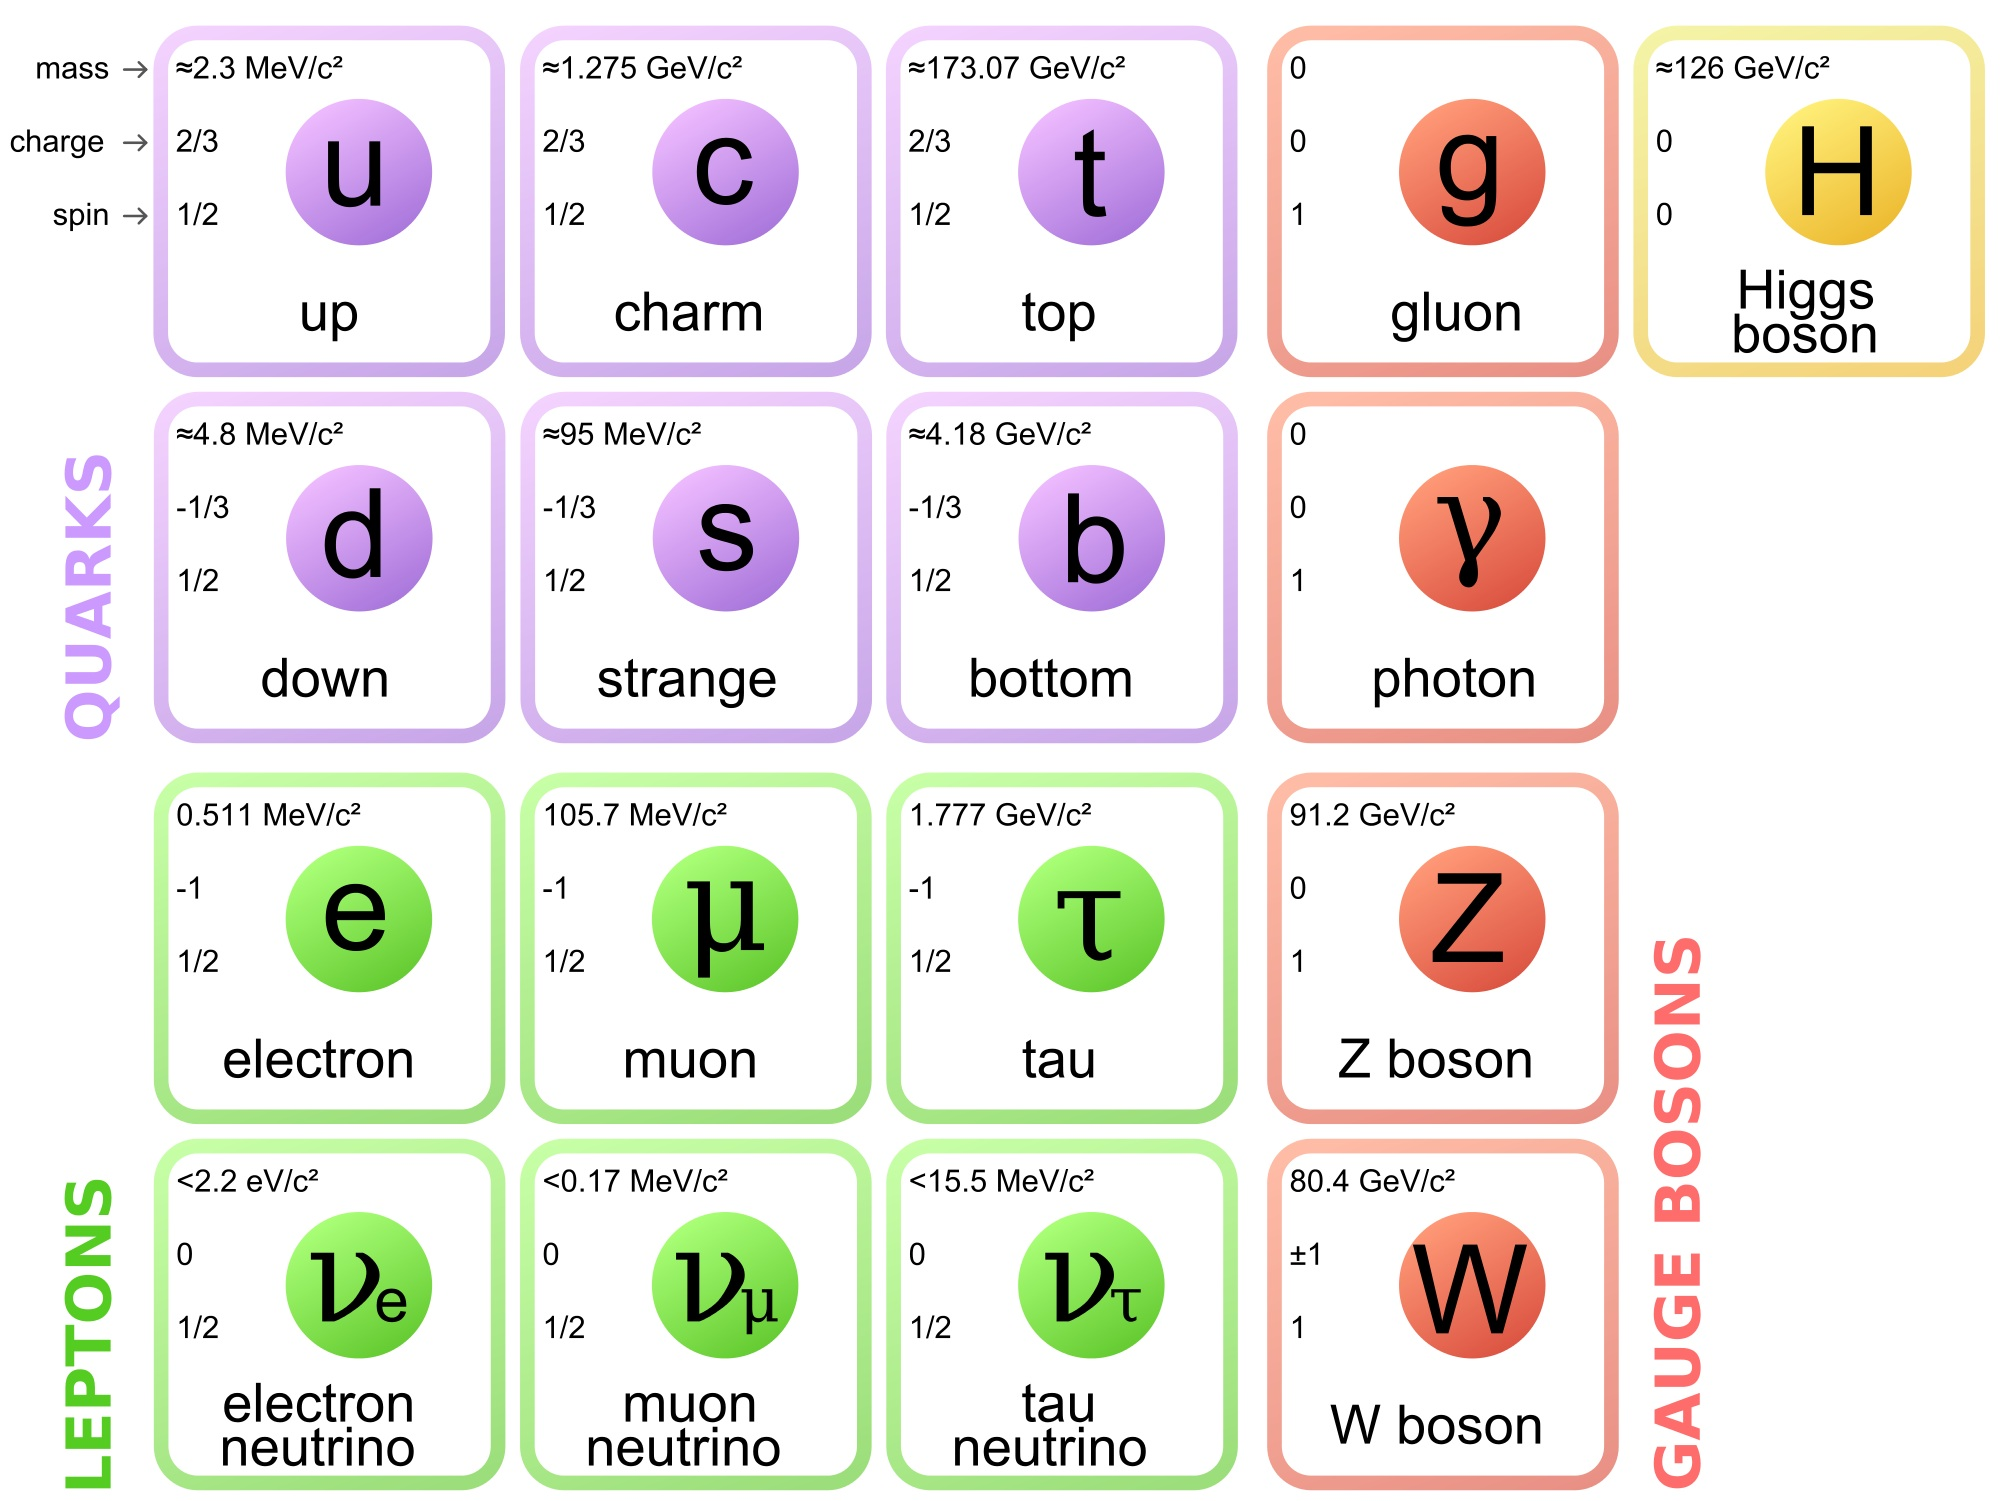
\includegraphics[clip, width=10cm]{fig/1/standardmodel.jpg}
  \caption{標準模型を構成する17種類の素粒子}
  \label{fig:標準模型}
\end{figure}


標準模型は多くの物理事象を説明することができているが、ダークマターの存在や階層問題などの多くの未解決問題が残されている。
この問題を解決するためには、標準模型を超える新しい物理が必要であり、この新物理を探索するための実験が世界中で行われている。

現在、新物理を探究するために世界中で様々なアプローチの実験が行われている。
このアプローチの一つとして、ジュネーブ郊外にある欧州原子核研究機構 (CERN) の地下に設置された Large Hadron Collider (LHC) を用いた高エネルギーの衝突実験がある。
この衝突実験の一つである LHC-ATLAS 実験では、LHC の衝突点に設置された ATLAS 検出器を用いて高エネルギーの陽子-陽子衝突によって生成される粒子を検出し、標準理論を構成する素粒子の精密測定や超対称性粒子の探索が行われている。

ATLAS実験では陽子を$40$ MHzの頻度で衝突させ、新物理探索を行っている。しかし、計算機リソースやデータ容量などの観点からこの高頻度での陽子-陽子衝突事象を全て保存することができない。
そこで、トリガーシステムを使った事象選別を行うことで膨大な量のデータから物理として興味のある事象を選別し、保存可能なデータ量まで事象を減らして保存している。
ATLAS実験は2段階のトリガーシステムを採用している。
1段目にはハードウェアベースの高速処理が可能な初段トリガー(L1)、2段目ではソフトウェアベースで精密処理が可能な後段トリガー(HLT)が実装されている。




<書くこと>
・Run-3及び高輝度においてルミノシティの増加に伴うトリガー性能の向上が重要な課題となっている。





